\chapter{Active and passive elements}

\modinfo{Directory}{PassiveElements}
\modinfo{Solvers}{\Idx{HeatSolve}}
\modinfo{Tools}{\Idx{ElmerGrid}, editor}
\modinfo{Dimensions}{2D}

\subsection*{Case definition}

This tutorial shows an example of using \Idx{passive elements} in
Elmer. This feature allows the activation and deactivation of
parts of the geometry during the simulation. This tutorial uses the
heat equation solver to demonstrate this capability. Use with other
solvers is analogous.

The geometry of the problem consists of two parts. The lower edge of
the lower part is held at constant temperature of 1 degrees. The upper
body is heated with a constant heating power. Between time steps 5 and
6 the two bodies are connected by two heat conductors, and the heat is
conducted from the higher body to the lower one. The goal of the
simulation is to model the temperature distribution in the system over
time. 

The problem is a pure heat transfer problem that may be solved
with \texttt{HeatSolve}. 


\subsection*{Solution Procedure}

The computational mesh is done with \texttt{ElmerGrid} in directory \texttt{tmesh} 
with the command 
%
\ttbegin
ElmerGrid 1 2 tmesh
\ttend
%
The command file may be written with a text editor. The file includes
the following information. 

The mesh directory is given in the header of the command file
%
\ttbegin
Header
  Mesh DB "." "tmesh"
End
\ttend
%
The simulation block of the command file defines, eg., the case to be time
dependent (transient) with 1 second time steps and altogether 15 time
intervals.  
%
\ttbegin
Simulation
  Max Output Level = 32
  Coordinate System = Cartesian 2D
  Simulation Type = Transient
  Timestepping Method = BDF
  BDF Order = 2
  Timestep Intervals = 15
  Timestep Sizes = 1
  Output Intervals = 1
  Steady State Max Iterations = 1
  Output Version Numbers = Logical True
  Output File = heat.res
  Post File = heat.ep
End
\ttend
%
The heat equation solver asks for the Stefan-Boltzmann constant that
gives the relationship between temperature and radiation power,
although radiation is not needed here. Let us define it anyway to
avoid warnings of missing parameters.
%
\ttbegin
Constants
  Stefan Boltzmann = 5.67e-8
End
\ttend
%
There are three bodies with the same equation but different material
properties. Body 3 is heated by a constant body force. Body 2 forms
the connecting parts of the system. An initial condition as well as a
body force is defined for this body. The body force contains the
initial deactivation, and later activation, of the connecting
part. Note that this part is included in the geometry all the time,
but the command file is used to define when they are included into the
simulation.
%
\ttbegin
Body 1
  Equation = 1
  Material = 1
End

Body 2
  Equation = 1
  Material = 2
  Body Force = 2
  Initial Condition = 1
End

Body 3
  Equation = 1
  Material = 1
  Body Force = 1
End
\ttend
%
The only solver is the heat solver (Solver 1)
%
\ttbegin
Equation 1
  Active Solvers = 1
End
\ttend
%
The initial condition for the initially passive elements is taken to
be 1 degrees; the same temperature than the colder part of the system
has as a boundary condition.
%
\ttbegin
Initial Condition 1
  Temperature = 1.0
End
\ttend
%
The heating power is defined to be 10 W/kg
%
\ttbegin
Body Force 1
  Heat Source = 10
End
\ttend
%
Now the passive condition for the connecting part is defined. When the
parameter \texttt{Temperature Passive} has a value larger than zero,
the current element is excluded from the solution, otherwise it is
included as a normal element. The parameter may depend on variables,
coordinates or time. Here it is defined to depend on time using a
tabular format.
%
\ttbegin
Body Force 2
  Temperature Passive = Variable Time
    Real
      0.0    1.0
      5.0    1.0
      5.2   -1.0
      8.0   -1.0
    End

End
\ttend
%
The material properties of the system are artificial. The following
three properties are needed for each material.
%
\ttbegin
Material 1
  Heat Capacity = 1
  Heat Conductivity = 1
  Density = 1
End

Material 2
  Heat Capacity = 10
  Heat Conductivity = 1
  Density = 1
End
\ttend
%
The heat equation is solved with an iterative method. The system is
linear, thus multiple non-linear iterations are not needed.
%
\ttbegin
Solver 1
  Equation = heat equation
  Linear System Solver = Iterative
  Linear System Iterative Method = BiCGStab
  Linear System Preconditioning = ILU0
  Linear System Max Iterations = 300
  Linear System Convergence Tolerance = 1.0e-6
  Linear System Abort Not Converged = Logical False
  Nonlinear System Max Iterations = 1
  Nonlinear System Convergence Tolerance = 1.0e-5
  Steady State Convergence Tolerance = 1.0e-5
End
\ttend
%
The boundary conditions are simple. The lower boundary of the lower
body is held at 1 degrees and the upper boundary of the upper body at
10 degrees.
%
\ttbegin
Boundary Condition 1
  Target Boundaries = 1

  Temperature = 1
End

Boundary Condition 2
  Target Boundaries = 4

  Temperature = 10
End
\ttend

After writing the command file is finished, the problem can be solved
by entering the command \texttt{ElmerSolver} on the command line. The
results can be examined with \texttt{ElmerPost}.


\subsection*{Results}

\begin{figure}
\begin{center}
  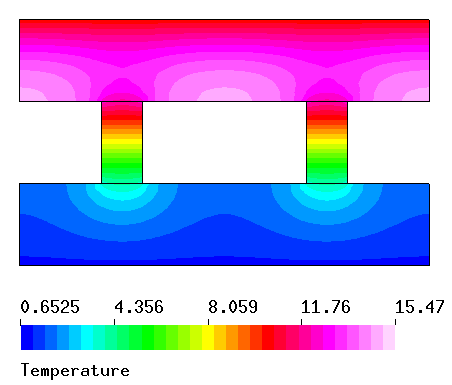
\includegraphics[height=0.5\textwidth]{heat.png}
\end{center}
\caption{Temperature distribution of the system at the final time
  instant (with spectral\_32 color map).}
\label{fig:temp_passive}
\end{figure}
 
With the given computational mesh the problem is solved in a few
seconds. The maximum and minimum temperatures in the system over the
whole simulation are 15.466 degrees and 0.6525 degrees
respectively. The maximum and minimum temperature at the final time
instant are 14.207 degrees and 1.000 degrees, respectively.  The
results at the time instant of 15 seconds are shown in
Fig.~\ref{fig:temp_passive}.


\subsection*{Notes}

For equations with more than one components (such as displacement for
Stress Analysis solver in 2D or 3D) the passive elements feature apply
to all the components. The feature is activated by defining, eg.,
\texttt{Displacement Passive} in the Body Force section. Note that
for Navier-Stokes equations one should use \texttt{Flow Solution
  Passive}, and that this affects the Pressure as well as the Velocity
components. 

However, when using multiple solvers, one can define some of them
passive and some of them active at the same time.


\hfill